\section{Initial Problem}
\label{sec:initproblem}

In a previous report we documented the work on a system that integrated wearables into a home automation environment in order to provide an interface for controlling devices that are connected to the Internet \cite{prespecialisation}. This report is based on the work done in our previous report.

In the previous report \cite[pp. 1-4]{prespecialisation} we presented \cref{fig:wearables-trend,fig:smarthomestrend}. The figures show an increasing trend in wearables and smart homes. Common for wearables and smart homes are that they are both involved in the concept of Internet of Things. As both concepts are predicted to be an increasing trend, it is interesting to combine the two in order to make a system that provides an interface for controlling a smart home using a wearable device.

\begin{figure}[!hbt]
  \centering
  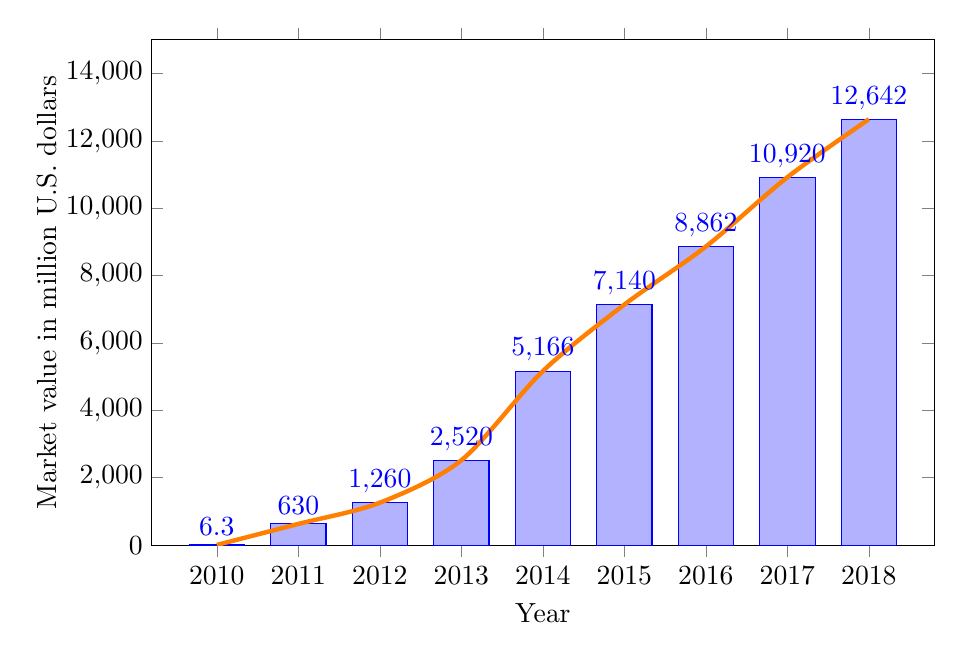
\begin{tikzpicture}
    \begin{axis}[
        height=8cm,
        width=0.95\textwidth,
        xlabel={Year},
        ylabel={Market value in million U.S. dollars},
        yticklabel style={align=right,inner sep=0pt,xshift=-0.3em},
        scaled y ticks = false,
        nodes near coords align={vertical},
        nodes near coords,
        xtick=data,
        symbolic x coords={2010, 2011, 2012, 2013, 2014, 2015, 2016, 2017, 2018},
        ymax=15000,
        ymin=0,
        ybar, 
        bar width=20pt
        ]
        \addplot coordinates {(2010, 6.3) (2011, 630) (2012, 1260) (2013, 2520) (2014, 5166) (2015, 7140) (2016, 8862) (2017, 10920) (2018, 12642)};
        \addplot [ultra thick,orange,line join=round,smooth, nodes near coords = ] coordinates {(2010, 6.3) (2011, 630) (2012, 1260) (2013, 2520) (2014, 5166) (2015, 7140) (2016, 8862) (2017, 10920) (2018, 12642)};
%        
    \end{axis}
\end{tikzpicture}
  \caption{Wearables trend based on sales and statistics. Data from \protect\cite{WEARABLESTRENDNUMBERS}.}
  \label{fig:wearables-trend}
\end{figure}

\begin{figure}[!hbt]
  \centering
  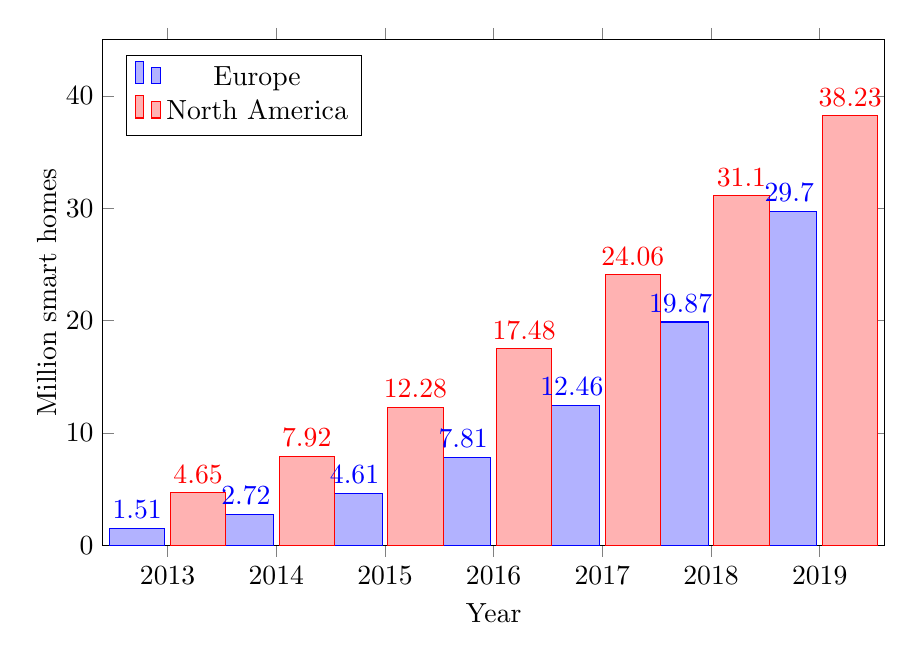
\begin{tikzpicture}
    \begin{axis}[
        height=8cm,
        width=0.95\textwidth,
        xlabel={Year},
        ylabel={Million smart homes},
        yticklabel style={align=right,inner sep=0pt,xshift=-0.3em},
        scaled y ticks = false,
        nodes near coords align={vertical},
        nodes near coords,
        xtick=data,
        symbolic x coords={2013, 2014, 2015, 2016, 2017, 2018, 2019},
        ybar,
        ymax=45,
        ymin=0,
        bar width=20pt,
        legend pos = north west,
        ]
        \addplot coordinates {(2013, 1.51) (2014, 2.72) (2015, 4.61) (2016, 7.81) (2017, 12.46) (2018, 19.87) (2019, 29.70)};        
        \addplot coordinates {(2013, 4.65) (2014, 7.92) (2015, 12.28) (2016, 17.48) (2017, 24.06) (2018, 31.10) (2019, 38.23)};
        \legend{Europe, North America}
        
        %Trend lines:
%        \addplot [ultra thick,orange,line join=round,smooth, nodes near coords = ] coordinates {(2013, 1.51) (2014, 2.72) (2015, 4.61) (2016, 7.81) (2017, 12.46) (2018, 19.87) (2019, 29.70)};
%        \addplot [ultra thick,orange,line join=round,smooth, nodes near coords = ] coordinates {(2013, 4.65) (2014, 7.92) (2015, 12.28) (2016, 17.48) (2017, 24.06) (2018, 31.10) (2019, 38.23)};
%        

    \end{axis}
\end{tikzpicture}
  \caption{Smart homes trend based on sales and statistics. Data from \protect\cite{SMARTHOMETREND}.}
  \label{fig:smarthomestrend}
\end{figure}

The definition of a \emph{smart home system} presented in \cite{SMARTHOMETREND} requires that the system uses a smartphone application or a web portal as a user interface. Therefore the numbers presented in \Cref{fig:smarthomestrend} does not include homes controlled solely by switches, timers, sensors and remote controls and as such the numbers would be higher if the definition was not as strict.

In order for a web portal or a smartphone application to provide meaningful functionality in a smart home system, the software should provide some mechanism for controlling or monitoring devices in the home. In order to do this, the devices are accessible using some technology for exchanging data, \eg~WiFi or Bluetooth. These devices are involved in the concept of Internet of Things. 

While not directly related to the concept of a smart home, a wearable device can play a role in a smart home. The wearable device can provide the application used for interacting with devices in the smart home.

Note that the definition of a smart home as presented in \cite{SMARTHOMETREND} does not include to which degree the smartphone application or web portal is involved in the smart home. A simple system including a smartphone app with a single button for turning a light on and off is regarded a \emph{smart home system}.

We accept the definition of a smart home presented in \cite{SMARTHOMETREND} and formulate it as shown in \Cref{def:smarthome} as it is sufficent for our use in that we are interested in replacing the smartphone app with an app running on wearable device.

\begin{definition}
\label{def:smarthome}
A smart home, is a home that can be controlled using a smartphone application or a web porta as a user interface.
\end{definition}

%%% Local Variables:
%%% mode: latex
%%% TeX-master: "../../master"
%%% End:
